\section*{Теоретическая справка}
\normalsize
\begin{itemize}
    \item{Уравнение ускоренного движения : $y = \upsilon_0 t+\frac{gt^2}{2}$}
    \item{Для n-го пролета между датчиком (расстояние между метками $l$): $nl = \upsilon_0 t_n + \frac{g_0t^2}{2}$}
    \item{Сила сопротивления: $F_{\text{сопр}} = C\pi r^2 \rho \upsilon^2 = mk\upsilon^2$}
    \item{Усредним силу сопротивления и получим формулу для $\Delta g: \Delta g = \frac{k{\upsilon_{\text{max}}}^2}{3}$ }
    \item{$g = g_0 - \Delta g$}
\end{itemize}
\section*{Экспериментальные данные}
\begin{table}[H]
    \begin{minipage}[c]{0.5\textwidth}
        \centering
        \begin{tabular}{|c|c|c|c|c|}
            \hline
            $r$, мм & $l$, cм & $m$, гр & $C$ & $\rho$, кг/м^3 \\ \hline
            15 & 38.8 & 106 & 0.2 & 1.2\\ \hline
        \end{tabular}
        \caption{Значениея необходимых величин}
        \label{tab:my_labe_1}
    \end{minipage}
    \begin{minipage}[c]{0.5\textwidth}
        \centering
        \begin{tabular}{|c|c|c|c|}
            \hline
            № & 1 & 2 & 3\\ \hline
            1 & 118.8 & 208.2 & 284.4\\ \hline
            2 & 120 & 210 & 287 \\\hline
            3 & 119.4 & 208.8 & 285.2 \\ \hline
        \end{tabular}
        \caption{Временя пролета первых трех меток}
        \label{tab:my_labe_2}
    \end{minipage}
\end{table}

\begin{figure}[ht]
  \centering
  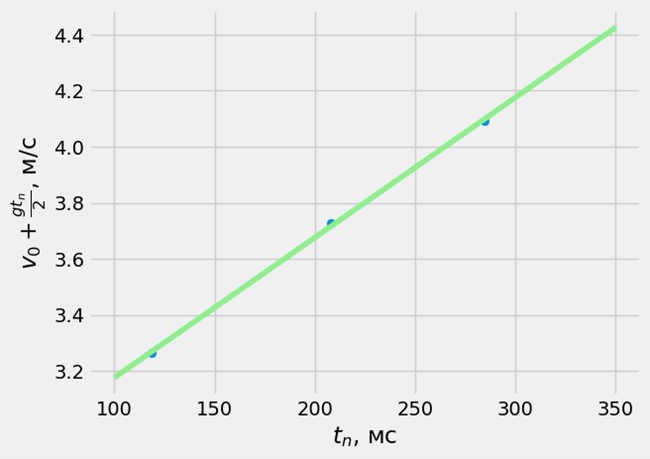
\includegraphics[width=8cm]{рис-1.png}
  \centering
  \caption{График, тангенс наклона которго равен $g_0$}
\end{figure}
$g_0 = 9.966$ м/c^2\\ [6pt]
$\upsilon_{\text{max}} \approx 6.3 \text{м/c} => \Delta g = 0.0022$ м/с^2\\[6pt]
С учетом поправки $\Delta g: g = 9.964$ м/с^2



